% Standalone regime-taxonomy flow diagram. Build: pdflatex flow.tex
\documentclass[border=4pt]{standalone}
\usepackage{tikz}
\usepackage{amsmath,amssymb}
\usetikzlibrary{arrows.meta,positioning}
\begin{document}
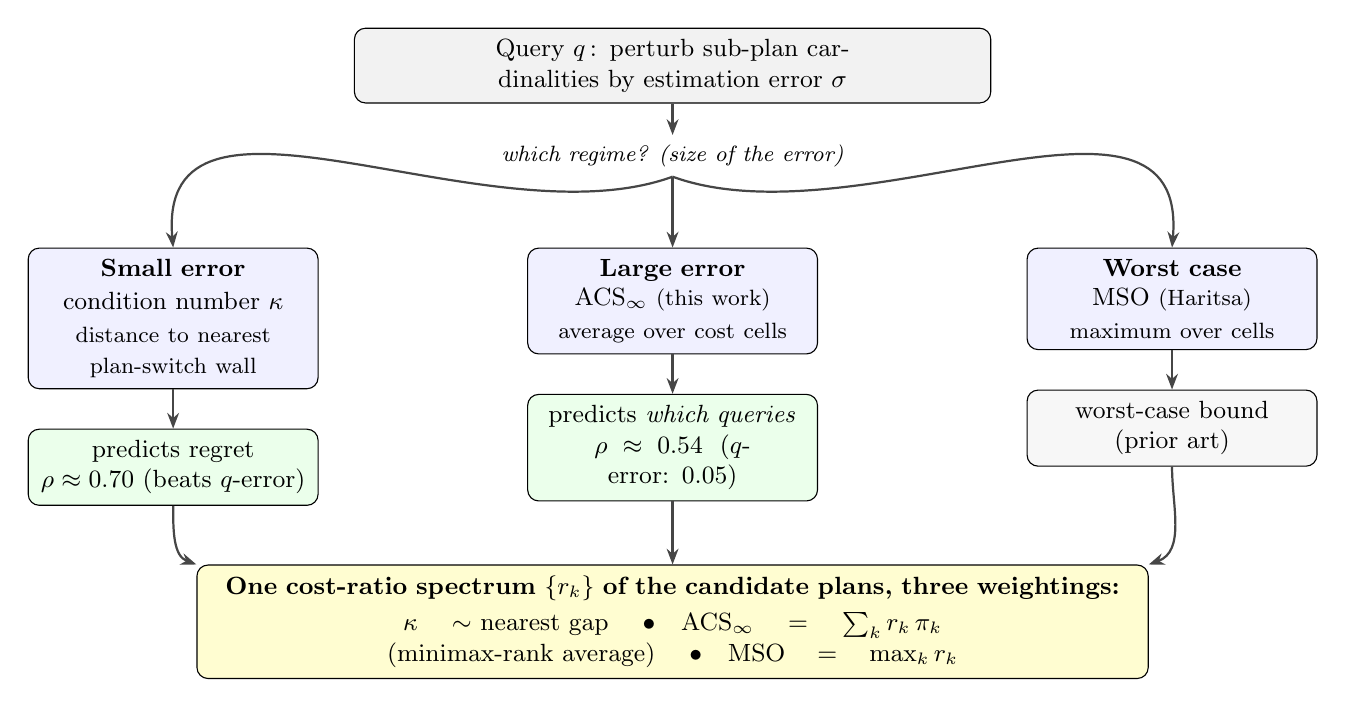
\begin{tikzpicture}[
  font=\small,
  box/.style={draw, rounded corners, align=center, inner sep=4pt, minimum height=9mm},
  reg/.style={box, fill=blue!6, text width=34mm},
  res/.style={box, fill=green!8, text width=34mm},
  arr/.style={-{Stealth[length=2mm]}, thick, gray!55!black}
]
\node[box, fill=gray!10, text width=78mm] (q)
  {Query $q$\,: perturb sub-plan cardinalities by estimation error $\sigma$};
\node[below=4mm of q, font=\itshape\footnotesize] (m) {which regime? (size of the error)};

\node[reg, below left=9mm and 22mm of m] (s)
  {\textbf{Small error}\\[1pt] condition number $\kappa$\\[1pt]
   \footnotesize distance to nearest plan-switch wall};
\node[reg, below=9mm of m] (l)
  {\textbf{Large error}\\[1pt] $\mathrm{ACS}_\infty$ \footnotesize(this work)\\[1pt]
   \footnotesize average over cost cells};
\node[reg, below right=9mm and 22mm of m] (w)
  {\textbf{Worst case}\\[1pt] MSO \footnotesize(Haritsa)\\[1pt]
   \footnotesize maximum over cells};

\node[res, below=5mm of s] (sr) {predicts regret\\ $\rho\approx0.70$ (beats $q$-error)};
\node[res, below=5mm of l] (lr) {predicts \emph{which queries}\\ $\rho\approx0.54$\ \ ($q$-error: $0.05$)};
\node[box, fill=gray!6, text width=34mm, below=5mm of w] (wr) {worst-case bound (prior art)};

\node[box, fill=yellow!18, text width=118mm, below=8mm of lr] (u)
  {\textbf{One cost-ratio spectrum $\{r_k\}$ of the candidate plans, three weightings:}\\[2pt]
   $\kappa\sim$ nearest gap \quad$\bullet$\quad
   $\mathrm{ACS}_\infty=\sum_k r_k\,\pi_k$ (minimax-rank average) \quad$\bullet$\quad
   $\mathrm{MSO}=\max_k r_k$};

\draw[arr] (q)--(m);
\draw[arr] (m.south) to[out=-160,in=95] (s.north);
\draw[arr] (m)--(l);
\draw[arr] (m.south) to[out=-20,in=85] (w.north);
\draw[arr] (s)--(sr);  \draw[arr] (l)--(lr);  \draw[arr] (w)--(wr);
\draw[arr] (sr.south) to[out=-90,in=160] (u.north west);
\draw[arr] (lr)--(u);
\draw[arr] (wr.south) to[out=-90,in=20] (u.north east);
\end{tikzpicture}
\end{document}
